%
% CSE Electronic Homework Template
% Last modified 8/23/2018 by Jeremy Buhler

\documentclass[11pt]{article}
\usepackage[left=0.7in,right=0.7in,top=1in,bottom=0.7in]{geometry}
\usepackage{fancyhdr} % for header
\usepackage{graphicx} % for figures
\usepackage{amsmath}  % for extended math markup
\usepackage{amssymb}
\usepackage[bookmarks=false]{hyperref} % for URL embedding
\usepackage[noend]{algpseudocode} % for pseudocode
\usepackage[plain]{algorithm} % float environment for algorithms

%%%%%%%%%%%%%%%%%%%%%%%%%%%%%%%%%%%%%%%%%%%%%%%%%%%%%%%%%%%%%%%%%%%%%%
% STUDENT: modify the following fields to reflect your
% name/ID, the current homework, and the current problem number

% Example: 
%\newcommand{\StudentName}{Jeremy Buhler}
%\newcommand{\StudentID{123456}

\newcommand{\StudentName}{Ming-Che Teng, Jingru Hu}
\newcommand{\StudentID}{466303, 466024}
\newcommand{\HomeworkNumber}{5}

%%%%%%%%%%%%%%%%%%%%%%%%%%%%%%%%%%%%%%%%%%%%%%%%%%%%%%%%%%%%%%%%%%%%%%%%
% You can pretty much leave the stuff up to the next line of %%'s alone.

% create header and footer for every page
\pagestyle{fancy}
\fancyhf{}
\lhead{\textbf{\StudentName}}
\chead{\textbf{\StudentID}}
\rhead{\textbf{Assignment \HomeworkNumber}}
\cfoot{\thepage}

% preferred pseudocode style
\algrenewcommand{\algorithmicprocedure}{}
\algrenewcommand{\algorithmicthen}{}

% ``do { ... } while (cond)''
\algdef{SE}[DOWHILE]{Do}{doWhile}{\algorithmicdo}[1]{\algorithmicwhile\ #1}%

% ``for (x in y ... z)''
\newcommand{\ForRange}[3]{\For{#1 \textbf{in} #2 \ \ldots \ #3}}

% these are common math formatting commands that aren't defined by default
\newcommand{\union}{\cup}
\newcommand{\isect}{\cap}
\newcommand{\ceil}[1]{\ensuremath \left\lceil #1 \right\rceil}
\newcommand{\floor}[1]{\ensuremath \left\lfloor #1 \right\rfloor}
\newcommand*{\Perm}[2]{{}^{#1}\!P_{#2}}%
\newcommand*{\Comb}[2]{{}^{#1}C_{#2}}%
\newcommand*{\Int}{\int\limits}
\usepackage{listings}
\usepackage{color}


\definecolor{dkgreen}{rgb}{0,0.6,0}
\definecolor{gray}{rgb}{0.5,0.5,0.5}
\definecolor{mauve}{rgb}{0.58,0,0.82}
\lstset{frame=tb,
  language=Java,
  aboveskip=3mm,
  belowskip=3mm,
  showstringspaces=false,
  columns=flexible,
  basicstyle={\small\ttfamily},
  numbers=none,
  numberstyle=\tiny\color{gray},
  keywordstyle=\color{blue},
  commentstyle=\color{dkgreen},
  stringstyle=\color{mauve},
  breaklines=true,
  breakatwhitespace=true,
  tabsize=3
}

%%%%%%%%%%%%%%%%%%%%%%%%%%%%%%%%%%%%%%%%%%%%%%%%%%%%%%%%%%%%%%%%%%%%%%

\begin{document}
\subsection * {Problems}

\begin{enumerate}

\item [\textbf{1.}]  

\textbf{BaggedTrees Implementation}

(a)

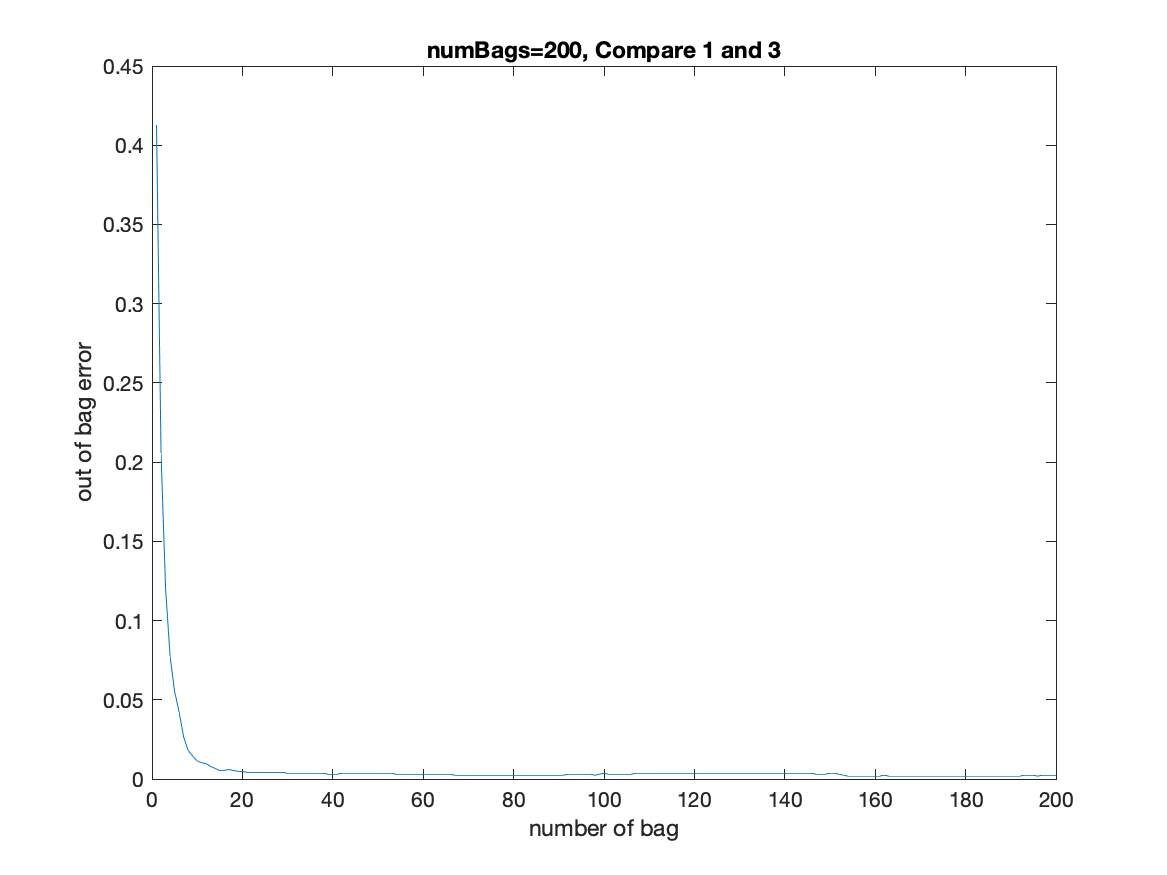
\includegraphics[scale = 0.45]{/Users/alexteng/Desktop/CSE417/h5_1.png}
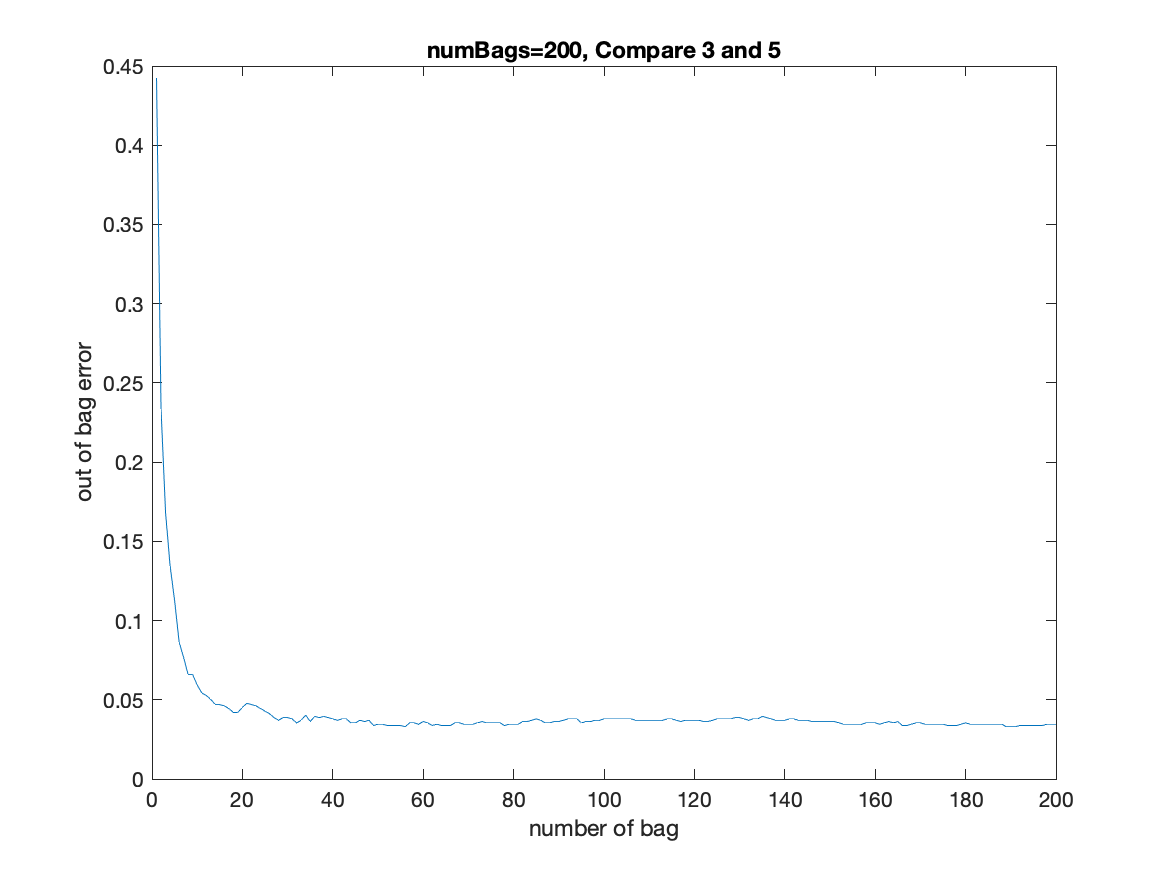
\includegraphics[scale = 0.45]{/Users/alexteng/Desktop/CSE417/h5_2.png}

The above graphs are the results that using random forest method to learn a tree for each bag and calculate the out-of-bag error in the group of 1 and 3 digits and 3 and 5 digits. 
As we can see, the out-of-bag error decreases with the number of bags increases. 


(b)

As we run the \texttt{OneThreeFive} file, the report is as follows, 

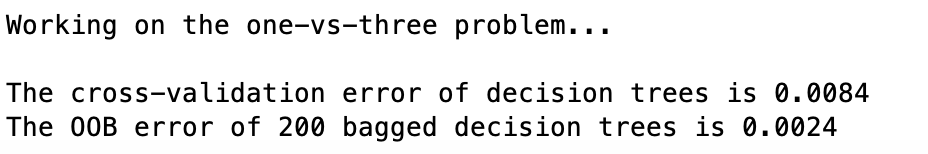
\includegraphics[scale = 0.5]{/Users/alexteng/Desktop/CSE417/H5_table.png}

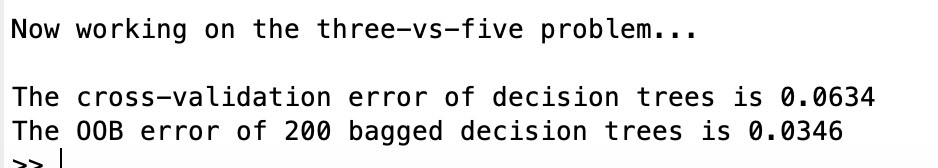
\includegraphics[scale = 0.5]{/Users/alexteng/Desktop/CSE417/H5_table2.png}

\begin{table}[h!]
\begin{center}
\caption{Results table of 1 v.s. 3 and 3 v.s. 5}
\label{tab:table1}
\begin{tabular}{l|c|r}
\hline
\text{ } & \text{1 v.s. 3} & \text{3 v.s. 5}\\
\text{Cross-Validation} & \text{0.0084} & \text{0.0634}\\
\text{Out-of-bag Error} & \text{0.0024} & \text{0.0346}\\
\end{tabular}
\end{center}
\end{table}


(c)

As we learn one decision tree from our training dataset, and use test dataset to estimate test error, the result is as follows, 

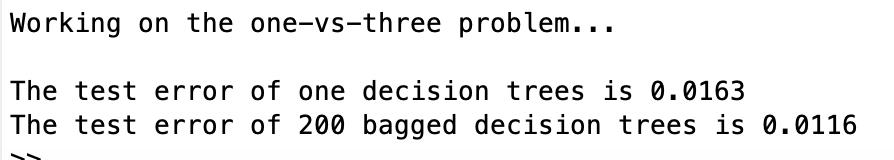
\includegraphics[scale=0.4]{/Users/alexteng/Desktop/CSE417/H5_table3.png}

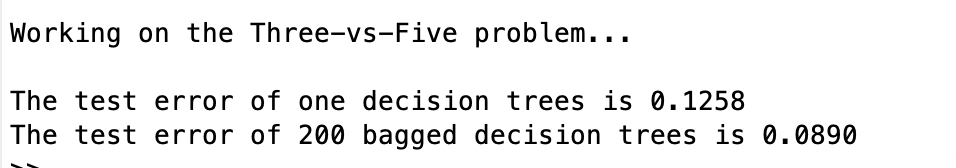
\includegraphics[scale=0.4]{/Users/alexteng/Desktop/CSE417/H5_table4.png}


\begin{table}[h!]
\begin{center}
\caption{Test Error of 1 v.s. 3 and 3 v.s. 5}
\label{tab:table1}
\begin{tabular}{l|c|r}
\hline
\text{ } & \text{1 v.s. 3} & \text{3 v.s. 5}\\
\text{One Tree} & \text{0.0163} & \text{0.1258}\\
\text{Ensemble of 200 Trees} & \text{0.0116} & \text{0.0890}\\
\end{tabular}
\end{center}
\end{table}

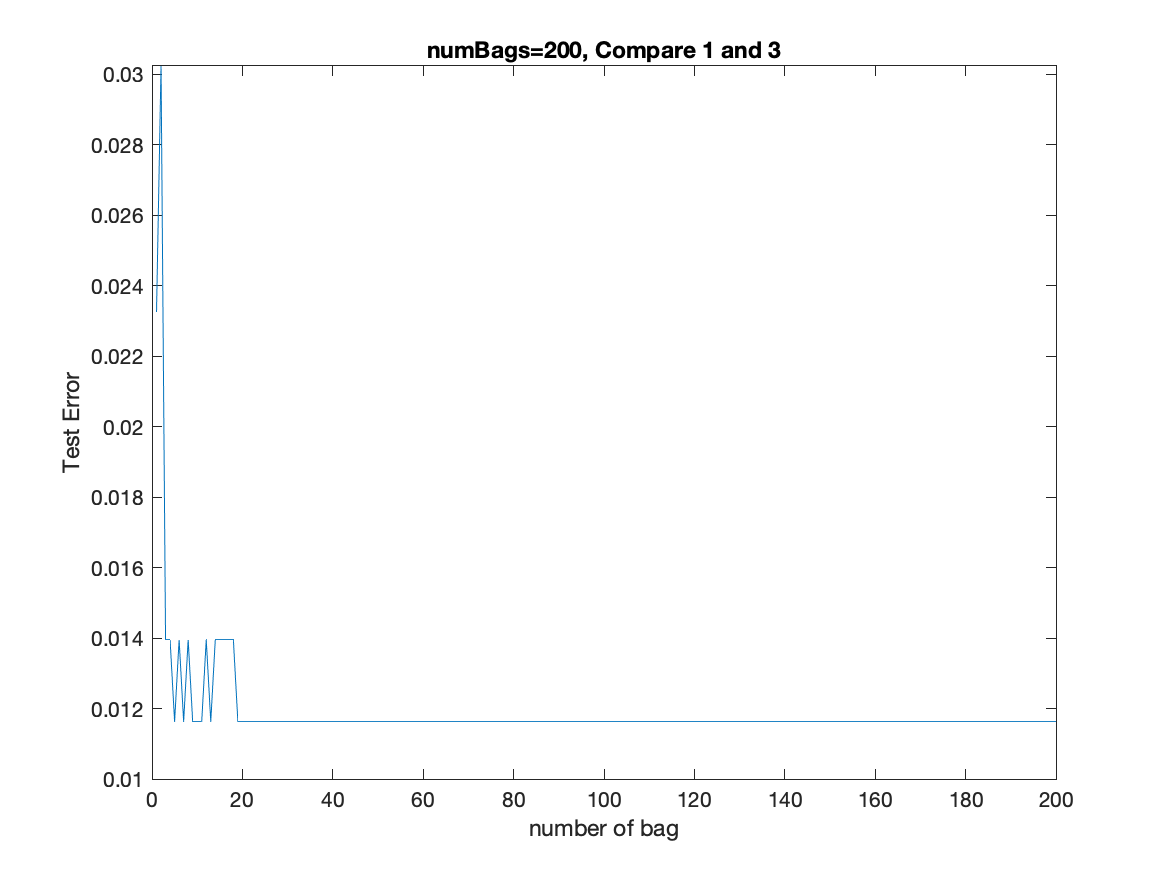
\includegraphics[scale = 0.45]{/Users/alexteng/Desktop/CSE417/h5_3.png}
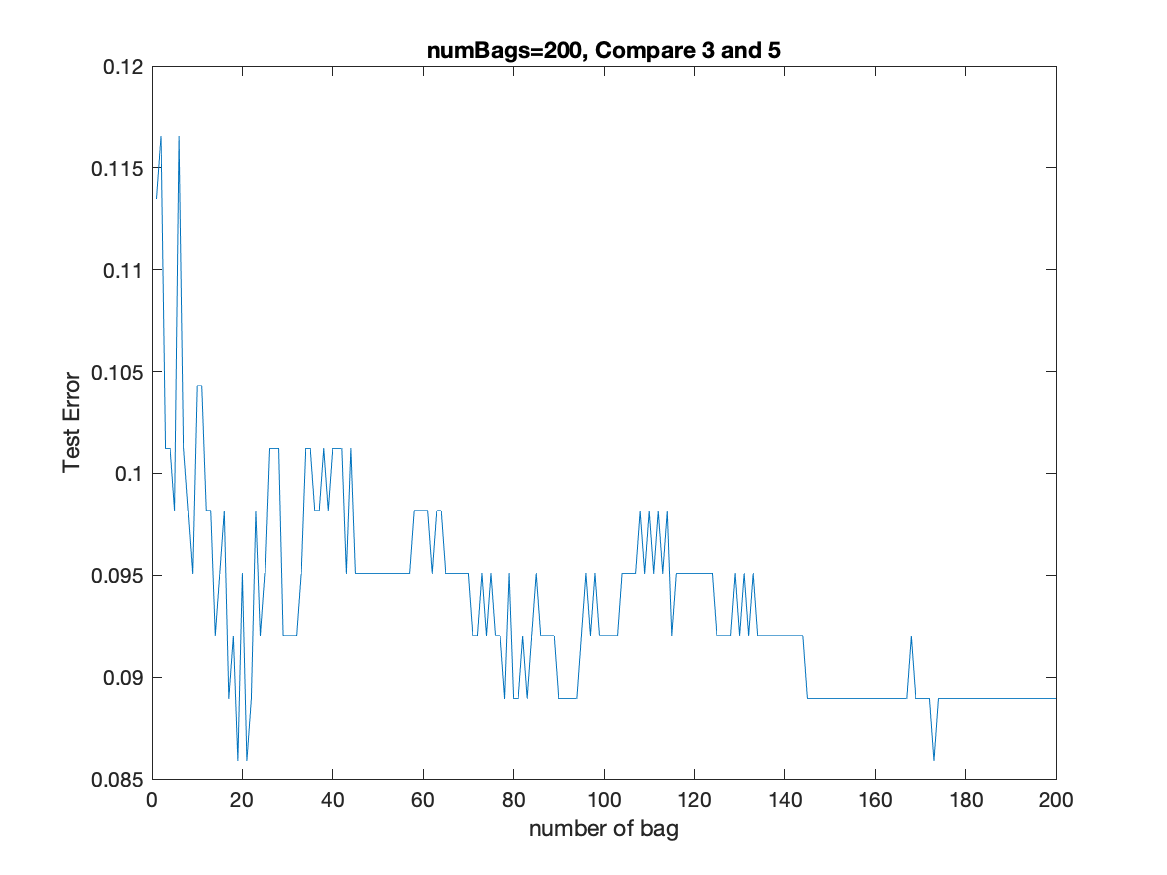
\includegraphics[scale = 0.45]{/Users/alexteng/Desktop/CSE417/h5_4.png}



(d)

For part (b), the result we got from cross-validation and bagging are different. It's because, bagging averages models in order to reduce the variance, while the cross-validation evaluate a number of surrogate models assuming they are all equivalent (good surrogate) for the actual model. The reason that cross-validation underperforms compared to bagging is because in a decision tree, using cross-validation could get a totally different tree each time we resample the training data, that means the variance is pretty high. And bagging is using multiple models to make more accurate predictions than any individual model. 

For part (c), which is an example that reinforce the point above, when we only have one decision tree, the test error can be enormously large. While we increased the number of bags, that could reduce the test error. 

In both out-of-bag error and test error, there's no significant to overfitting.

\end{enumerate}

\pagebreak

\subsection*{Problems}
\begin{enumerate}

\item[\textbf{2.}]

\textbf{Adaboost}

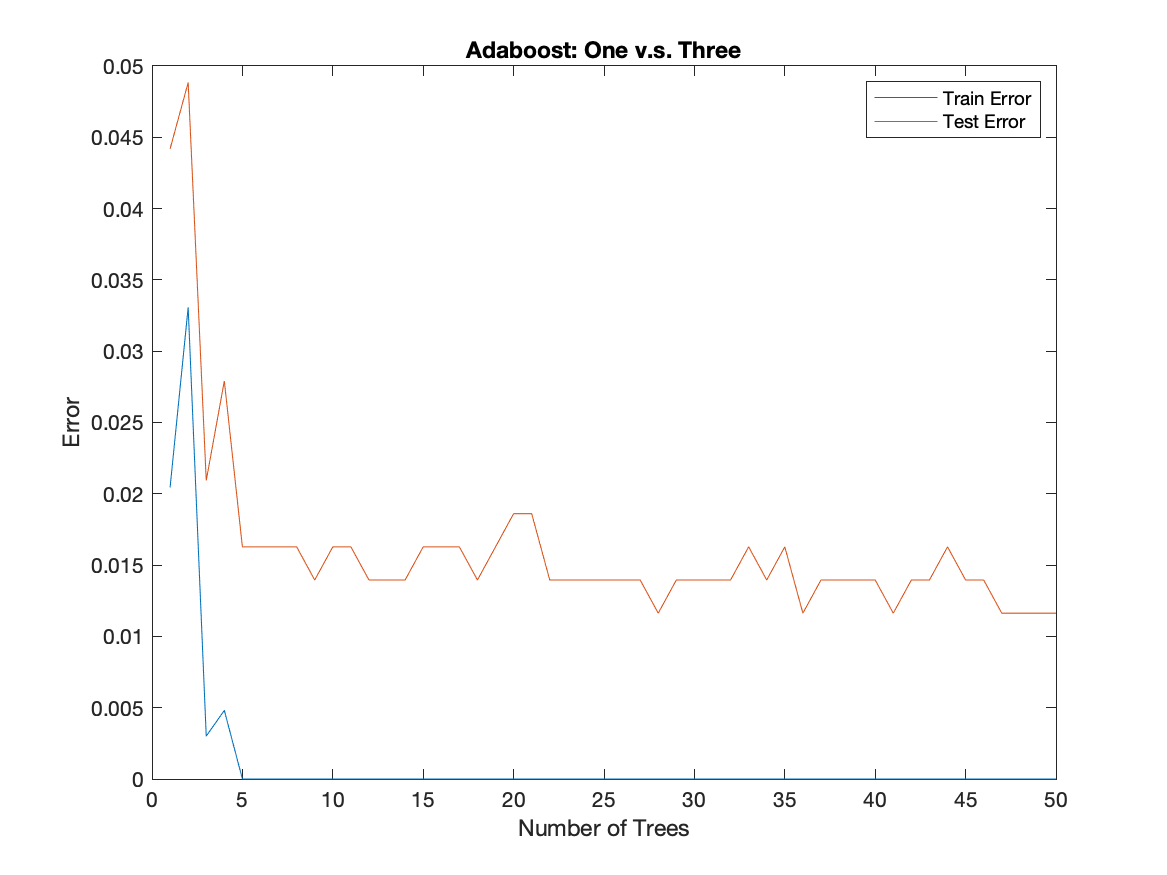
\includegraphics[scale = 0.45]{/Users/alexteng/Desktop/CSE417/HW5_5.png}
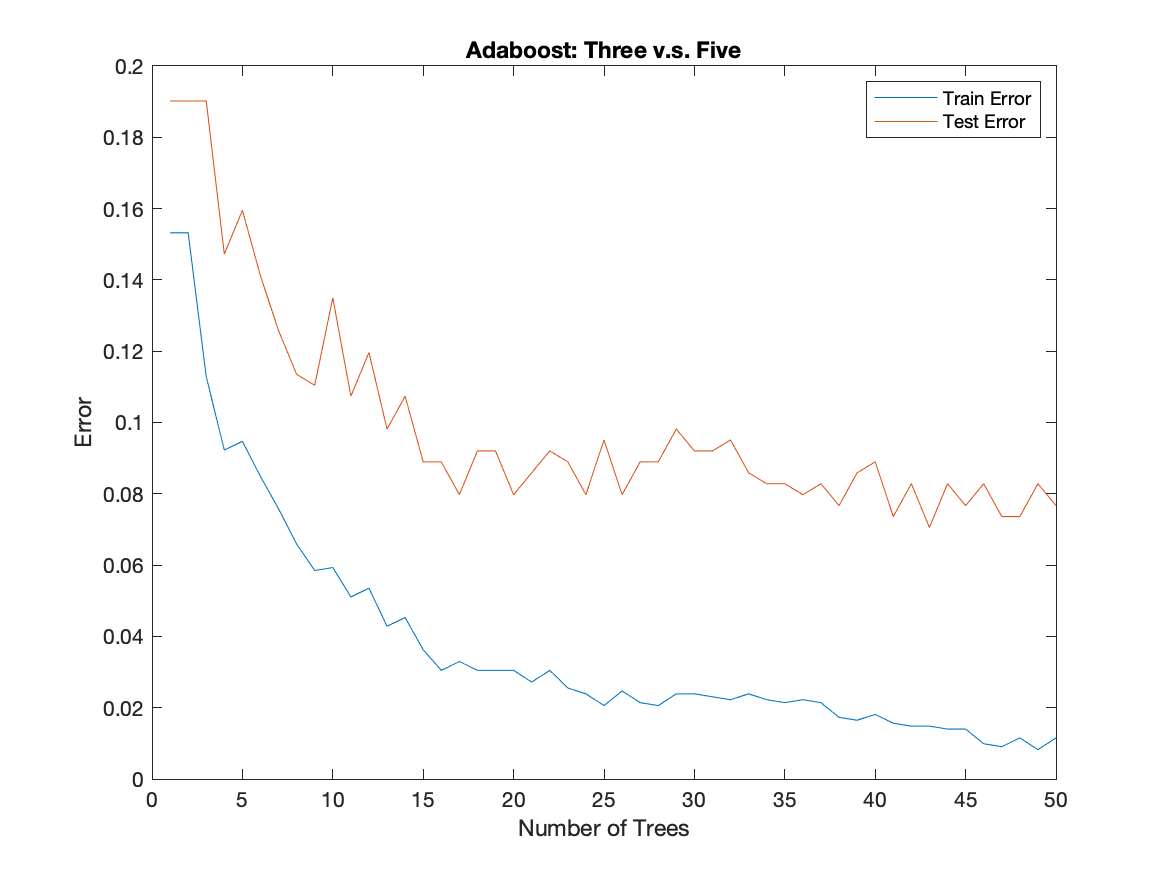
\includegraphics[scale = 0.45]{/Users/alexteng/Desktop/CSE417/HW5_6.png}

Adaboost is an algorithm that's to combine multiple weak learner into a stronger one. Each tree only uses one feature to do the split, that we call a stump, and there are a bunch of stumps and each stump has different importance and each time we split, we're going to focus more on the misclassified data points by increasing the weight on misclassified data points to let the next stump to adjust according to the sample rate. Basically, we use Gini index to decide which feature we're going to use to split our data at each depth, and by updating the sample weight, we can calculate weighted Gini Index to determine which variable is going to be used to split the next stump.  The weighted Gini Index would put more emphasis on correctly classifying the samples that are misclassified by the previous stump since the samples have larger weight.  The alternative is we can use sample weights to create a new dataset that reflects those weight. 

After a briefly intro to the Adaboost, we can explain the result in a more intuitive way.

What we can observe is that in both cases, \texttt{One v.s. Three} and \texttt{Three v.s. Five}, the training error is lower than test error. This is pretty intuitive, after all, we use our training dataset to build our decision tree so we can expect the training error would be lower than the error that comes from by using a different dataset, that is, test dataset. 

The other fact is, by increasing the number of trees we can observe the error decreases. It should not be surprise as a tree with more depth, the higher chance that our tree could correctly classify our data point. And by using Adaboost, since we're focusing on the misclassified data points, there's a chance that we may suffer from overfitting since the algorithm will put more weight on the misclassified data points and that would affect how we grow our tree. 

\end{enumerate}
\pagebreak


\subsection*{Collaboration Statement}

I collaborate this assignment with Jingru Hu, 466024, jingruhu@wustl.edu.

\end{document}